\chapter{User manual}


\section{The web interface}
You can connect to your PDR instance using any web browser. Just navigate to your server and enter your username and password.

\subsection{Login}
\begin{figure}[h]
	\centering
	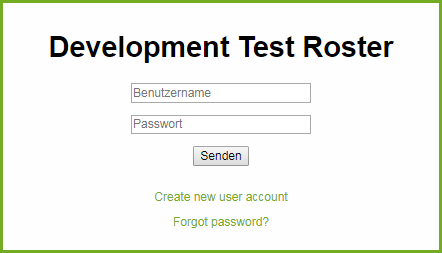
\includegraphics[width=.3\linewidth]{{images/en_GB/login.php}.png}
	\caption{Login page}
\end{figure}
The login page shows the name of the application. You are prompted to enter your username and password.
If you do not have an account yet, you can \menu{Create a new user account}.
If you have an account, but forgot about your password, or want to change it, you can click on \menu{Forgot password?}.


\subsection{Create new user account}
\begin{figure}[ph]
	\centering
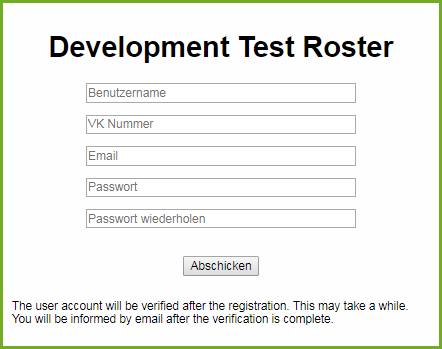
\includegraphics[width=0.4\linewidth]{{images/en_GB/register.php}.png}
	\caption{Register new user page}
\end{figure}
Choose a user name, enter your employee id and your email. Pick a secure password.

The account will be inactive until an administrator activates it. The main administrator is informed via email regarding the registration.

New users can only be created for existing employees. New employees are created by an administrator. 

\subsection{Lost password}
\begin{figure}[h]
    \centering
    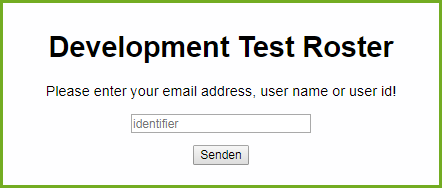
\includegraphics[width=.3\linewidth]{{images/en_GB/lost_password.php}.png}
    \caption{Lost password page}
\end{figure}
The lost password page shows the name of the application. You are prompted to enter either your username, id or your email-address at your option.
After you submit the form, an email is sent to your stored email address.
In that email you will find a link, which will lead you to the password change page.
\subsubsection{Lost password recovery}
\begin{figure}[ph]
    \centering
    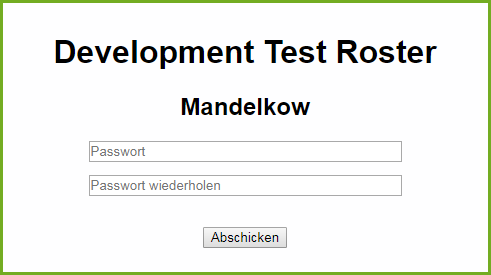
\includegraphics[width=0.3\linewidth]{{images/en_GB/reset-lost-password.php}.png}
    \caption{Lost password recovery page}
\end{figure}
The lost password recovery page shows the name of the application and your user name. You are prompted to enter a new password twice.


\subsection{Navigation}
\begin{figure}[ph]
	\centering
	
\includegraphics[width=0.8\linewidth]{{images/en_GB/navigation}.png}
	\caption{Navigation bar}
	\label{img_navigation_bar}
\end{figure}
By default, the PDR web interface opens a menu containing 5 tiles.
You can navigate to:
\begin{itemize}
\item Roster week table view 
\includegraphics[height=2em]{../img/week_2}
\item Roster daily view 
\includegraphics[height=2em]{../img/day}
\item Roster employee view 
\includegraphics[height=2em]{../img/employee_2}
\item Overtime  
\includegraphics[height=2em]{../img/watch_overtime}
\item Absence 
\includegraphics[height=2em]{../img/absence}
\end{itemize}

\subsubsection{The navigation bar}
In the top there is a navigation bar containing hyperlinks to nearly all the pages of PDR. Hover the mouse over an entry to open the submenus (\autoref{img_navigation_bar}).
\begin{multicols}{3}
\begin{description}
    \item \menu{Weekly view > .. }
    \begin{description}
        \item \menu{.. > Weekly table}
        \item \menu{.. > Weekly images}
    \end{description}
    \item \menu{Daily view > .. }
    \begin{description}
    \item \menu{.. > Daily input}
    \item \menu{.. > Daily output}
    \item \menu{.. > Principle roster daily}
    \end{description}
    \columnbreak
    \item \menu{Employee > .. }
    \begin{description}
    \item \menu{.. > Roster employee}
    \item \menu{.. > Principle roster employee}
    \end{description}
    \item \menu{Overtime > ..}
    \begin{description}
    \item \menu{.. > Overtime input}
    \item \menu{.. > Overtime output}
    \item \menu{.. > Overtime overview}
    \end{description}
    \item \menu{Absence > ..}
    \begin{description}
    \item \menu{.. > Absence input}
    \item \menu{.. > Absence annual plan}
    \item \menu{.. > Absence monthly plan}
    \end{description}
    \columnbreak
    \item \menu{Administration > ..}
    \begin{description}
    \item \menu{.. > Attendance list}
    \item \menu{.. > Saturday list}
    \item \menu{.. > Marginal employment hours list}
    \item \menu{.. > Upload deployment planning}
    \item \menu{.. > Human resource managament}
    \item \menu{.. > Branch managament}
    \item \menu{.. > User managament}
    \item \menu{.. > Configuration}
    \item \menu{.. > phpMyAdmin}
    \end{description}
\end{description}
\end{multicols}
\subsection{Roster week table view}
\begin{figure}[h]
	\centering
	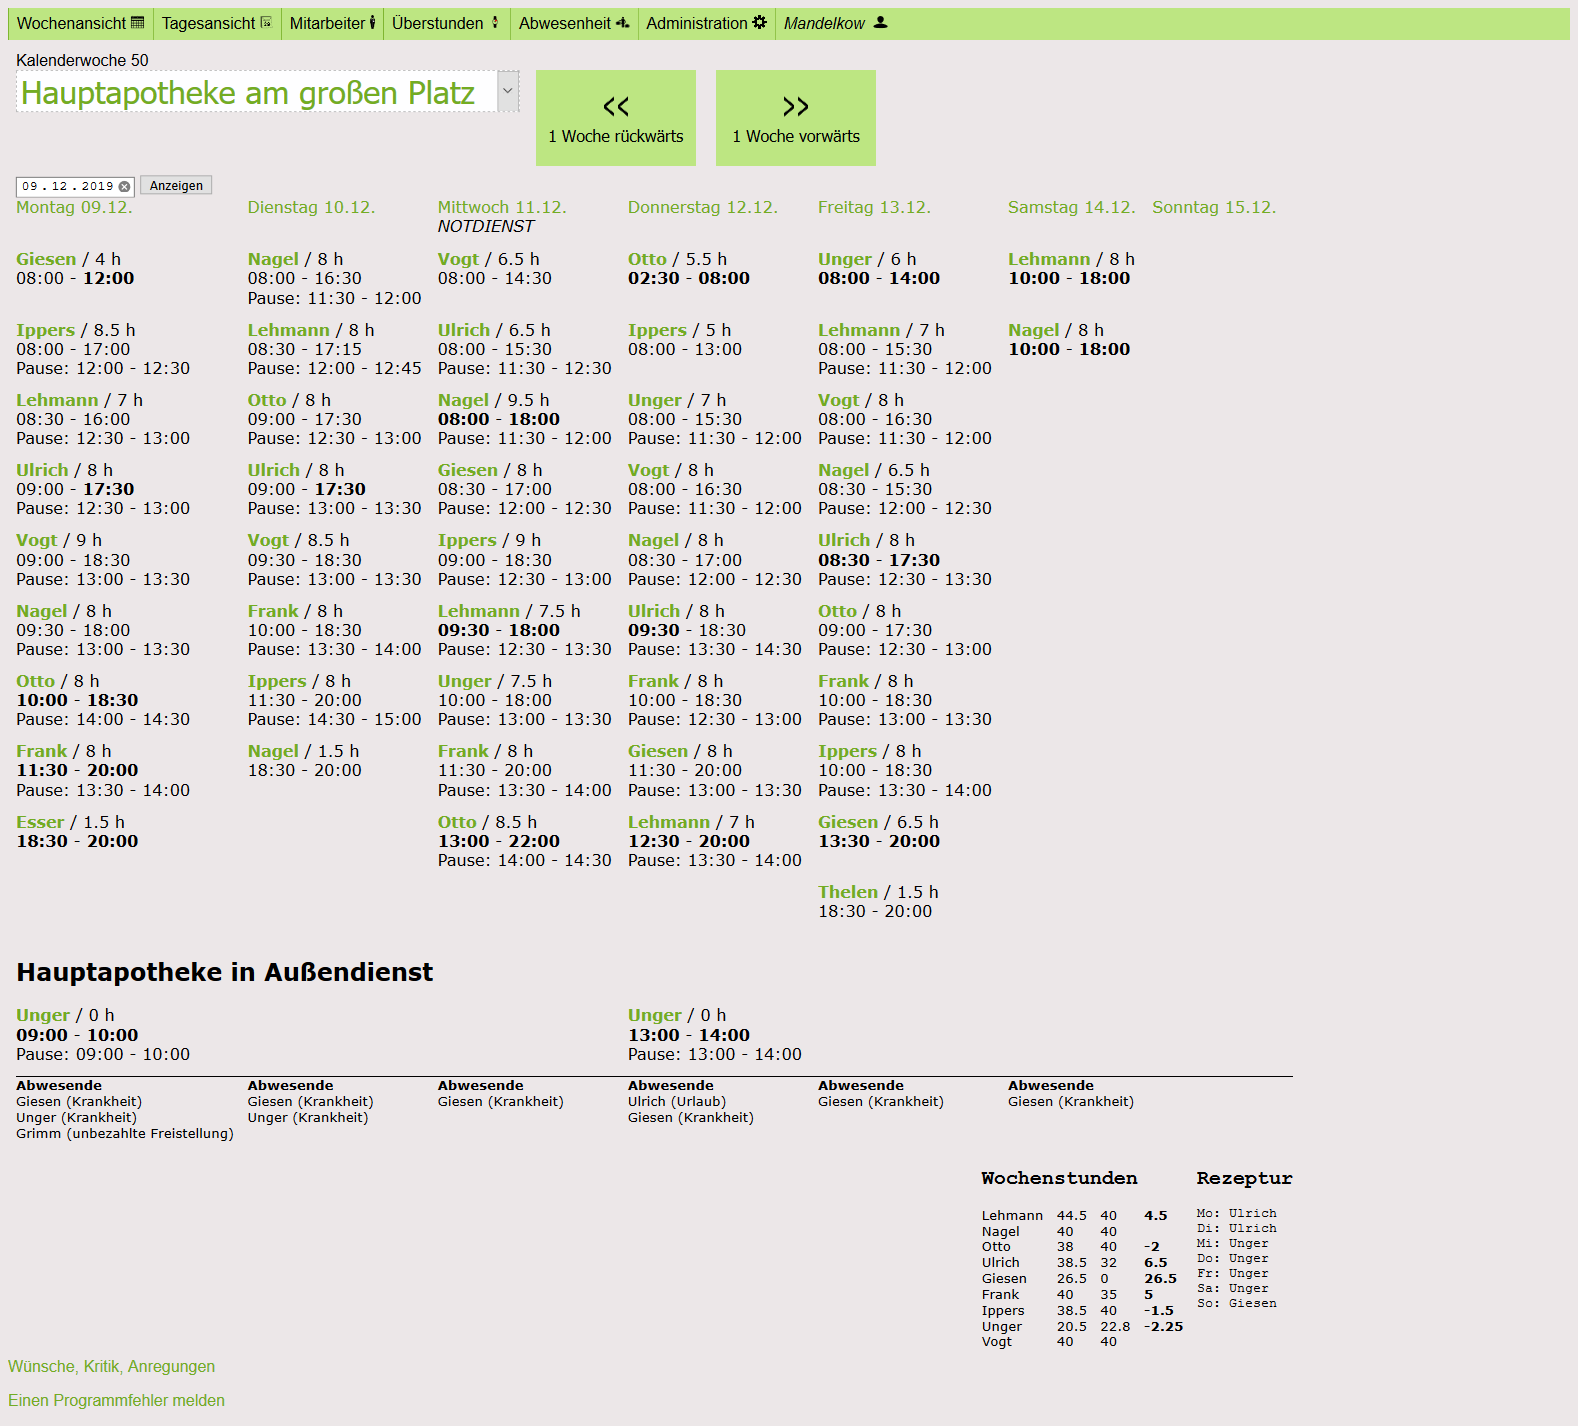
\includegraphics[width=0.8\linewidth]{{images/en_GB/roster-week-table.php}.png}
	\caption{Roster week table view, excerpt without task rotation and weekly working hours}
	\label{img_roster_week_table_view}
\end{figure}

The roster week table view shows the roster of a chosen week and branch (\autoref{img_roster_week_table_view}). If employees of the branch are working in an other branch, then those are shown below.
The table foot contains the information about absent employees and their reason of absence.

The date can be chosen by direct input. It can also be shifted by one week backwards or forwards by pressing \keys{\ctrl + \shift + \arrowkeyright} or \keys{\ctrl + \shift + \arrowkeyleft} respectively.

\subsection{Roster daily view}
\subsubsection{Read only}
In the daily roster view there is a table, a bar plot and a histogram reflecting the roster (\autoref{img_roster-day-read}).

\begin{figure}[h]
	\centering
	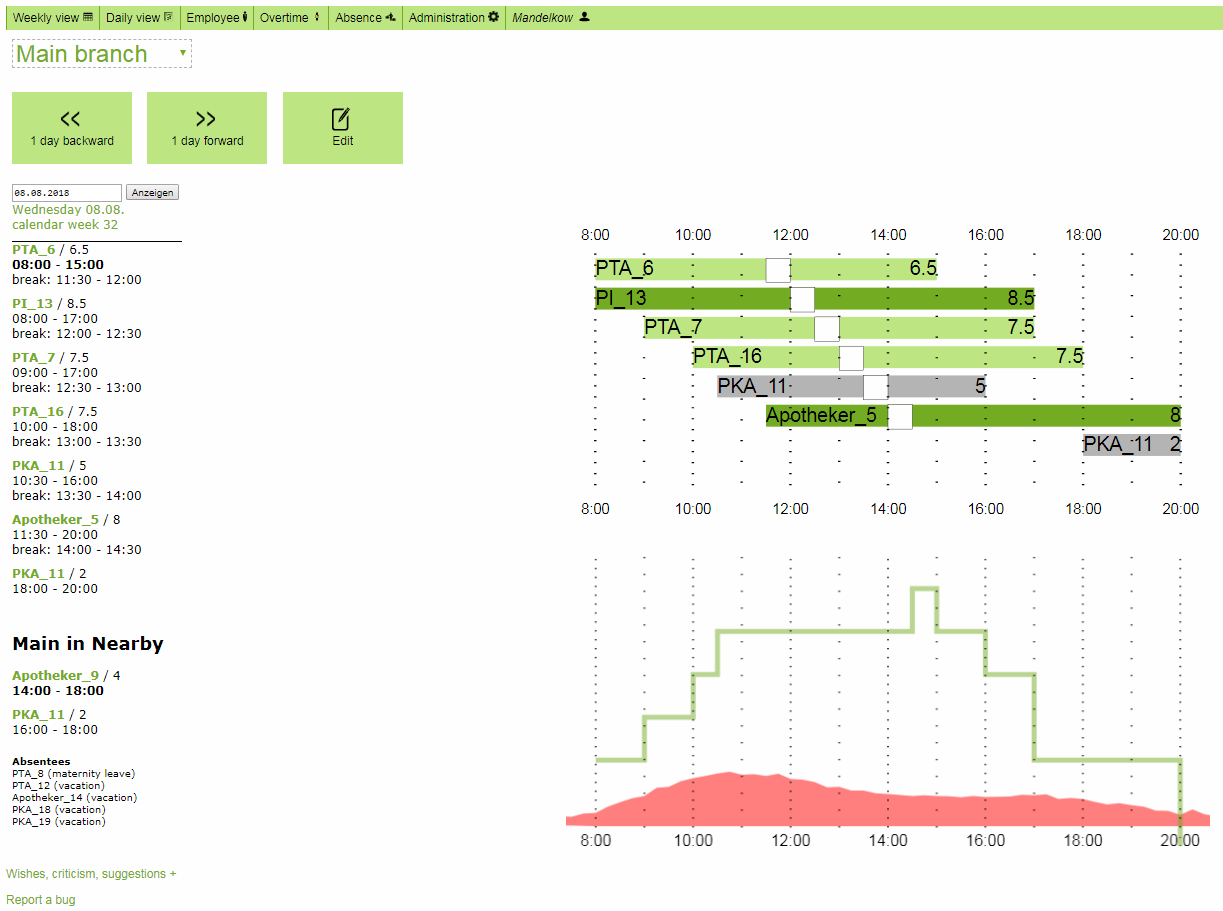
\includegraphics[width=0.8\linewidth]{{images/en_GB/roster-day-read.php}.png}
	\caption{Roster day view}
	\label{img_roster-day-read}
\end{figure}

The roster table lists all the employees scheduled in the chosen branch on the one chosen day. For every entry there is the employee id and last name, the working hours, the start and end of duty and the time of the lunch break, if any.

If an employee, that is primarily scheduled in the chosen branch, works in an other branch, then this entry is shown in the table at the bottom.
An employee may have more than one entrie per day. This allows divided working time to be stored.
If employees are absent, these absences are displayed in the table footer.


The roster bar plot shows the flow of employees coming and going. Each bar represents one entry. It reaches from the start of duty to its end. A white rectangle on the bar shows the time of the lunch break. The color of the bars is dependent on the profession of the employee. Pharmacists and Pharmazieingenieure \footnote{specific eastern german profession, see \url{https://de.wikipedia.org/wiki/Pharmazieingenieur}} are colored in dark green, while Pharmacy technicians are colored in light green. Other employees (non-pharmaceutical personnel) are colored in grey.

The histogram plot shows a red area and a green line. The red area shows the expected amount of work (measured in packages per 15 minutes), while the green line represents the amount of working employees on any given time.


\subsubsection{Edit}
The edit page looks quite similar to the read only view (\autoref{img_roster-day-edit}). 

\begin{figure}[h]
	\centering
	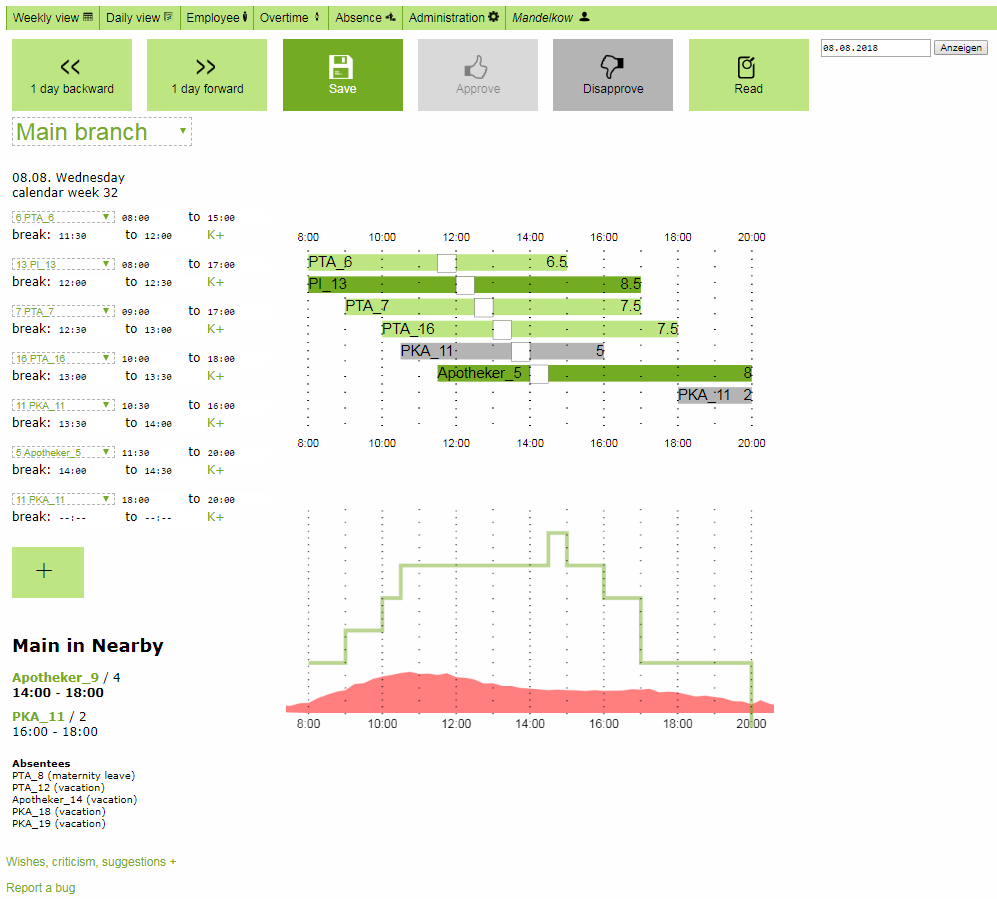
\includegraphics[width=0.8\linewidth]{{images/en_GB/roster-day-edit.php}.png}
	\caption{Roster day view with edit privileges}
	\label{img_roster-day-edit}
\end{figure}

The roster is examined for errors. If any issues occur, then errors, warnings or information will be shown in the top right area.
The examination includes:
\begin{itemize}
    \item overlap of shifts for the same employee (Error)
    \item sufficient employee count (Warning, hardcoded at least two employees)
    \item attendance of at least one pharmacist at any time (Error).
    \item attendance of at least one person able to carry out goods receipt (Warning).
    \item scheduling of absent employees (Error)
    \item non-scheduling of non-absent employees (Warning)
\end{itemize}

Only one break can be inserted per entry. If more breaks have to be assigned, then it is possible to enter multiple entries for the same employee.

\subsection{Roster employee view}
The employee view is similar to the weekly view, but only one employee is shown (\autoref{img_roster-employee-table}).

\begin{figure}[h]
	\centering
	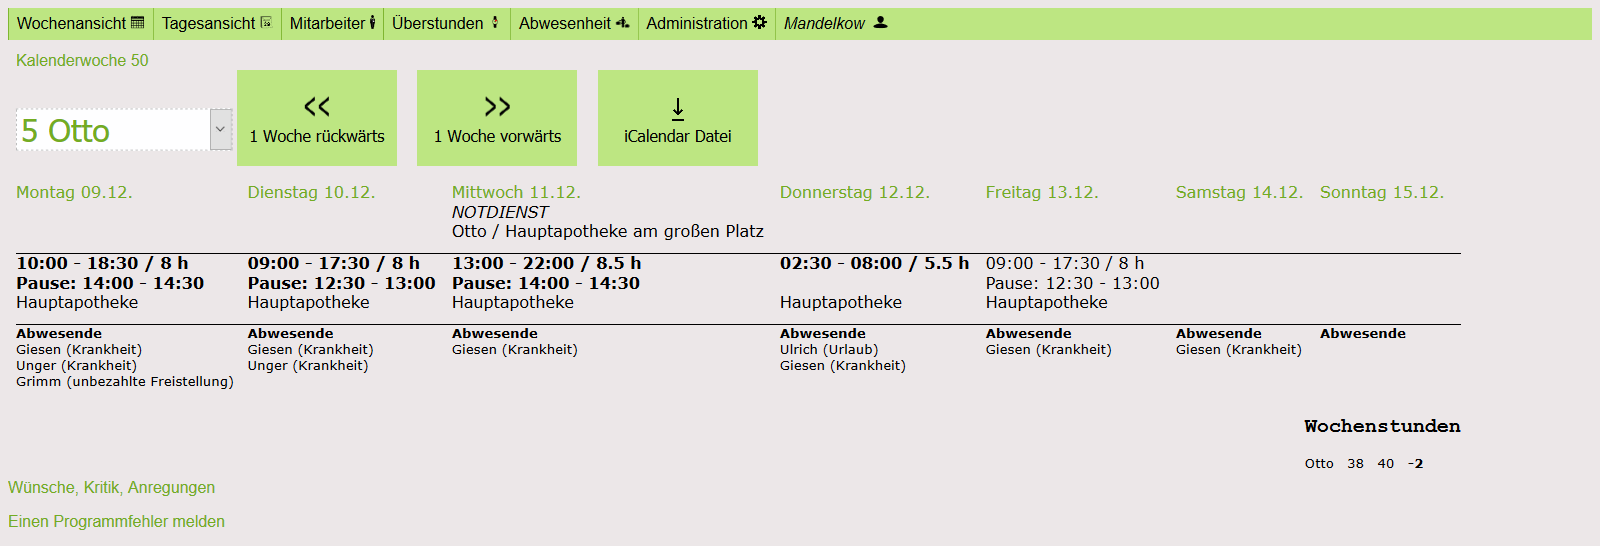
\includegraphics[width=0.8\linewidth]{{images/en_GB/roster-employee-table.php}.png}
	\caption{Employee view}
	\label{img_roster-employee-table}
\end{figure}

An iCalendar file can be downloaded. See \autoref{section-calendar-api}~\nameref{section-calendar-api} for details.

\subsection{Principle roster daily}
A principle recurring roster can be saved. In the simplest case it is a list of the start and end of duty for all the employees.
Every weekday is listed separately, and so are the branches.

It is possible to create alternating weeks. For example an employee might work on an A-Week and a B-Week. On A-Weeks she might regularly start at 08:00 in the morning on Mondays, while on B-Weeks she starts at 10:00.



\subsection{Overtime}
\subsection{Absence}
There are four views to the absence data.
\begin{itemize}
\item Employee view readonly
\item Employee view edit
\item Monthly table
\item Year overview
\end{itemize}
In the \emph{Employee view readonly} there is a select element to choose the employee to view. There is a button to switch to the edit view.
And there is a table containing the absence data. The columns are start and end of the absence, reason of absence and number of days.
There is a distinct list of possible reasons ( vacation,
        remaining holiday,
       sickness,
        sickness of child,
        unpaid leave of absence,
        paid leave of absence,
        parental leave and
        maternity leave).
The number of days of absence is calculated for a 5 day week. Absences on saturdays and sundays are registered but not counted. The same applys for holidays.



\section{Calendar API}\label{section-calendar-api}
It is possible to read the roster data from PDR in form of iCalendar files.
These files can be used with all major calendar applications on desktops and smartphones.
This API is by no means a full implementation of the webdav standard. It is not even an implementation of the CalDAV protocol.
Just point your browser to the following URL:
\url{https://YOURHOSTNAME/YOUR/FOLDER/webdav.php}


The options are:
\begin{description}
	\item \lstinline|employee_id|
	The employee id of the user from whom the roster should be given.
	Any user can get the roster of every employee.
	(default = the logged in user)
	\item \lstinline|date_string|
	A date in the format YYYY-MM-DD
	(default = today)
	\item \lstinline|days_into_the_future|
	The number of days that should be in the calendar file.
	(default = 30)
	\item \lstinline|create_valarm|
	Create an alarm (\lstinline|ACTION:DISPLAY|) on your device.
	(default = 0)
	\begin{itemize}
        \item 0 = no alarm
        \item 1 = alarm 30 minutes before beginning of duty
        \item 2 = alarm on the end of duty
        \item 4 = alarm when the lunch break starts
        \item 8 = alarm when the lunch break ends
        \item 11 = 1+2+8 = alarm for start and end of duty and for end of lunch, but not for start of lunch
    \end{itemize}	
\end{description}	

In order to get the roster of the week starting on 17.12.2018 for the employee number 5 you would use the following url:
\url{https://YOURHOSTNAME/YOUR/FOLDER/webdav.php?employee_id=5&date_string=2018-12-17&days_into_the_future=6}

\subsection{Automatically import iCalendar files with "iCal Import/Export CalDAV Pro"}
Automatic import of iCalendar files into Android smartphones has been tested with 
"iCal Import/Export CalDAV Pro" (3,59 EUR). There are probably other apps, that can do the same.

\begin{figure}[hbtp]
    \centering
    \begin{minipage}{0.45\textwidth}
        \centering
	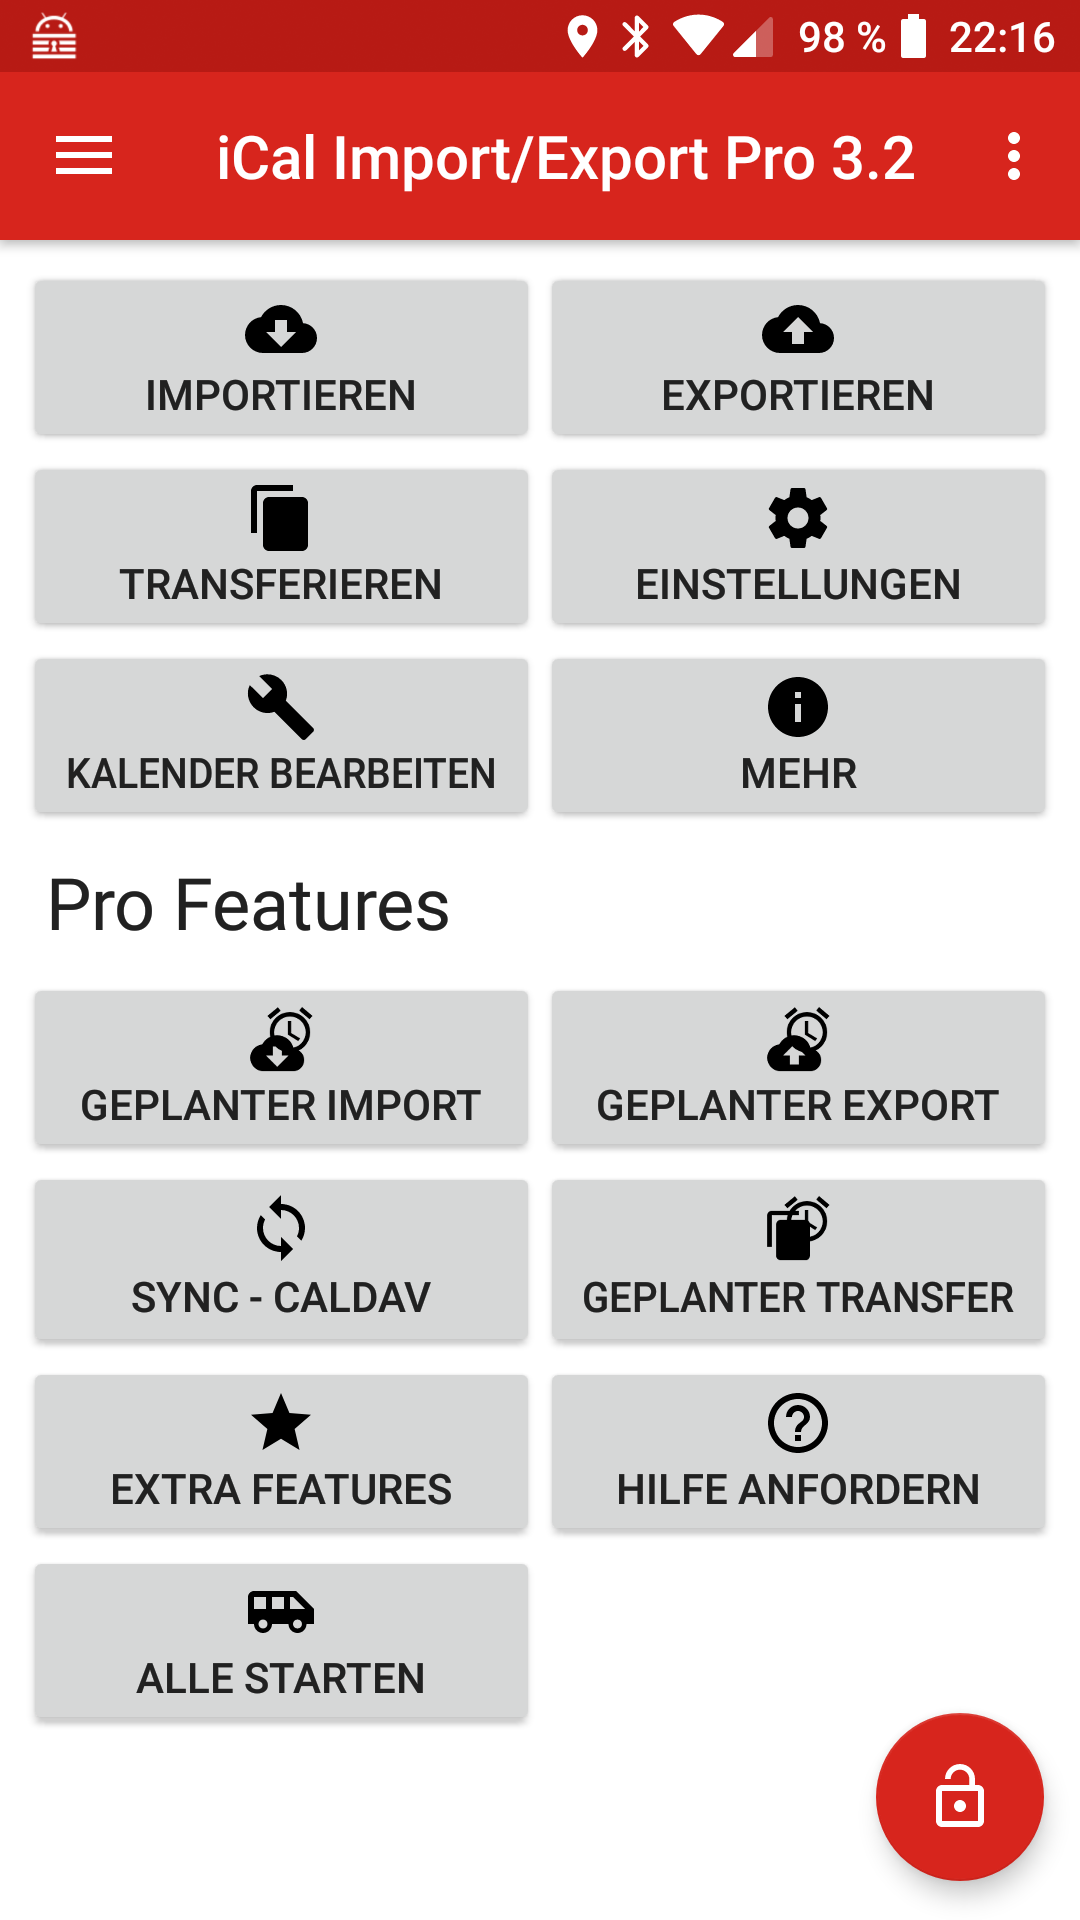
\includegraphics[width=0.9\textwidth, height=0.3\textheight, keepaspectratio=true]{{images/de_DE/iCalendar_import_0.png}}
	\caption{iCal main menu}
    \end{minipage}\hfill
    \begin{minipage}{0.45\textwidth}
        \centering
	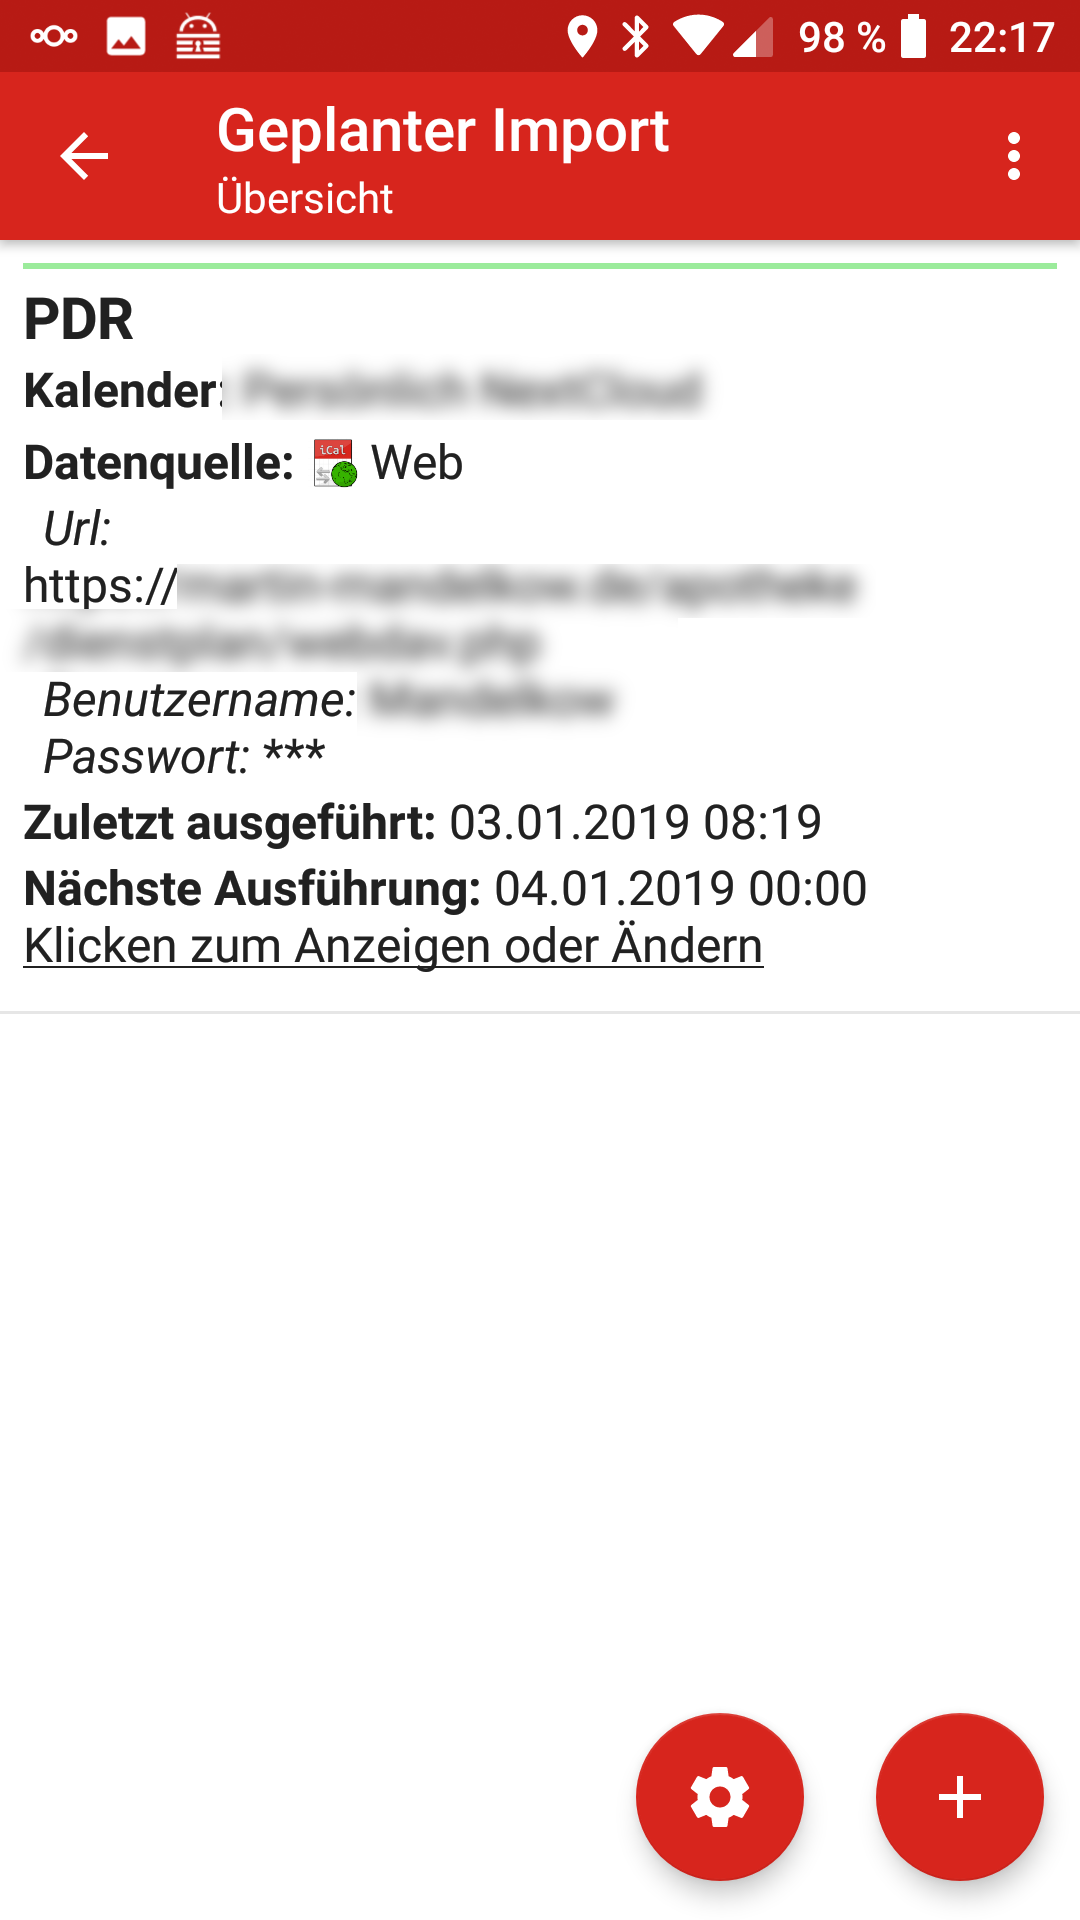
\includegraphics[width=0.9\textwidth, height=0.3\textheight, keepaspectratio=true]{{images/de_DE/iCalendar_import_1.png}}
	\caption{iCal planned imports}
    \end{minipage}
    \vfill
    \centering
    \begin{minipage}{0.45\textwidth}
        \centering
	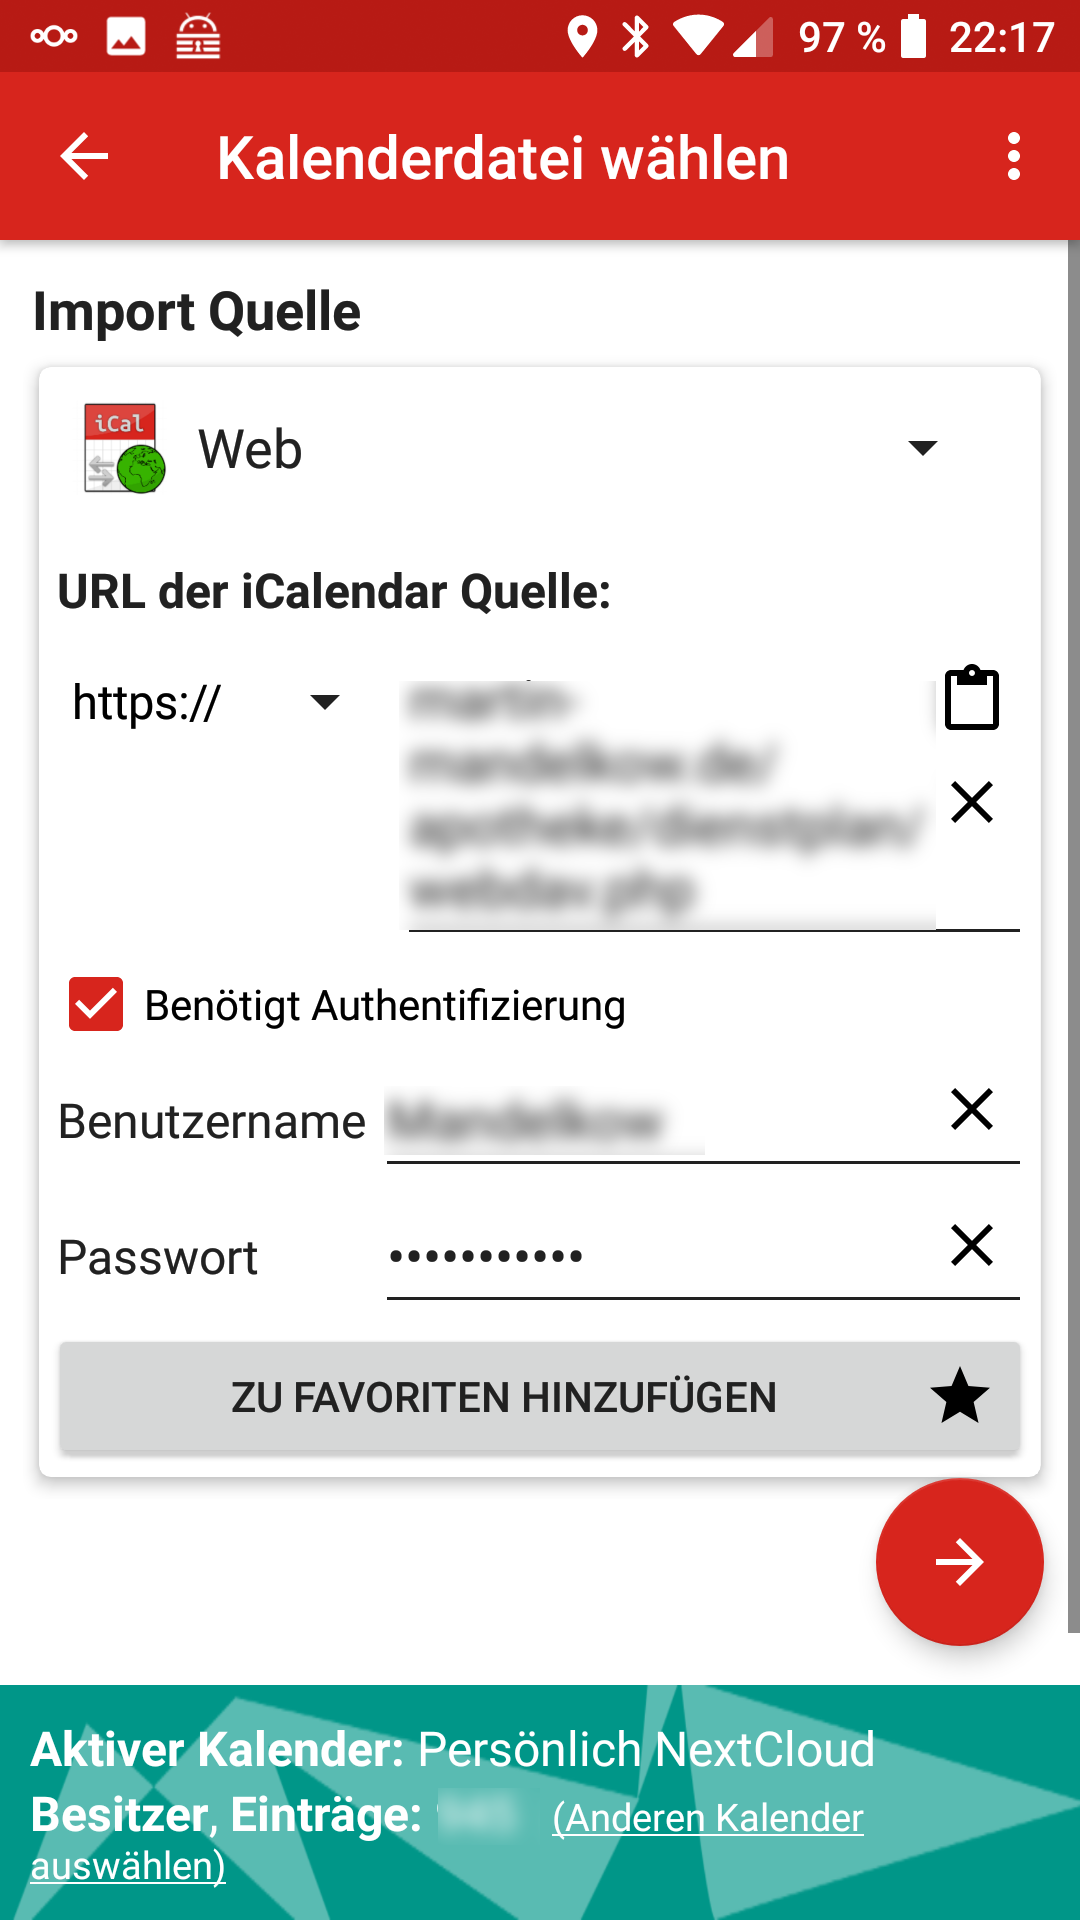
\includegraphics[width=0.9\textwidth, height=0.3\textheight, keepaspectratio=true]{{images/de_DE/iCalendar_import_2.png}}
	\caption{iCal adding a new import source}
    \end{minipage}\hfill
    \begin{minipage}{0.45\textwidth}
        \centering
	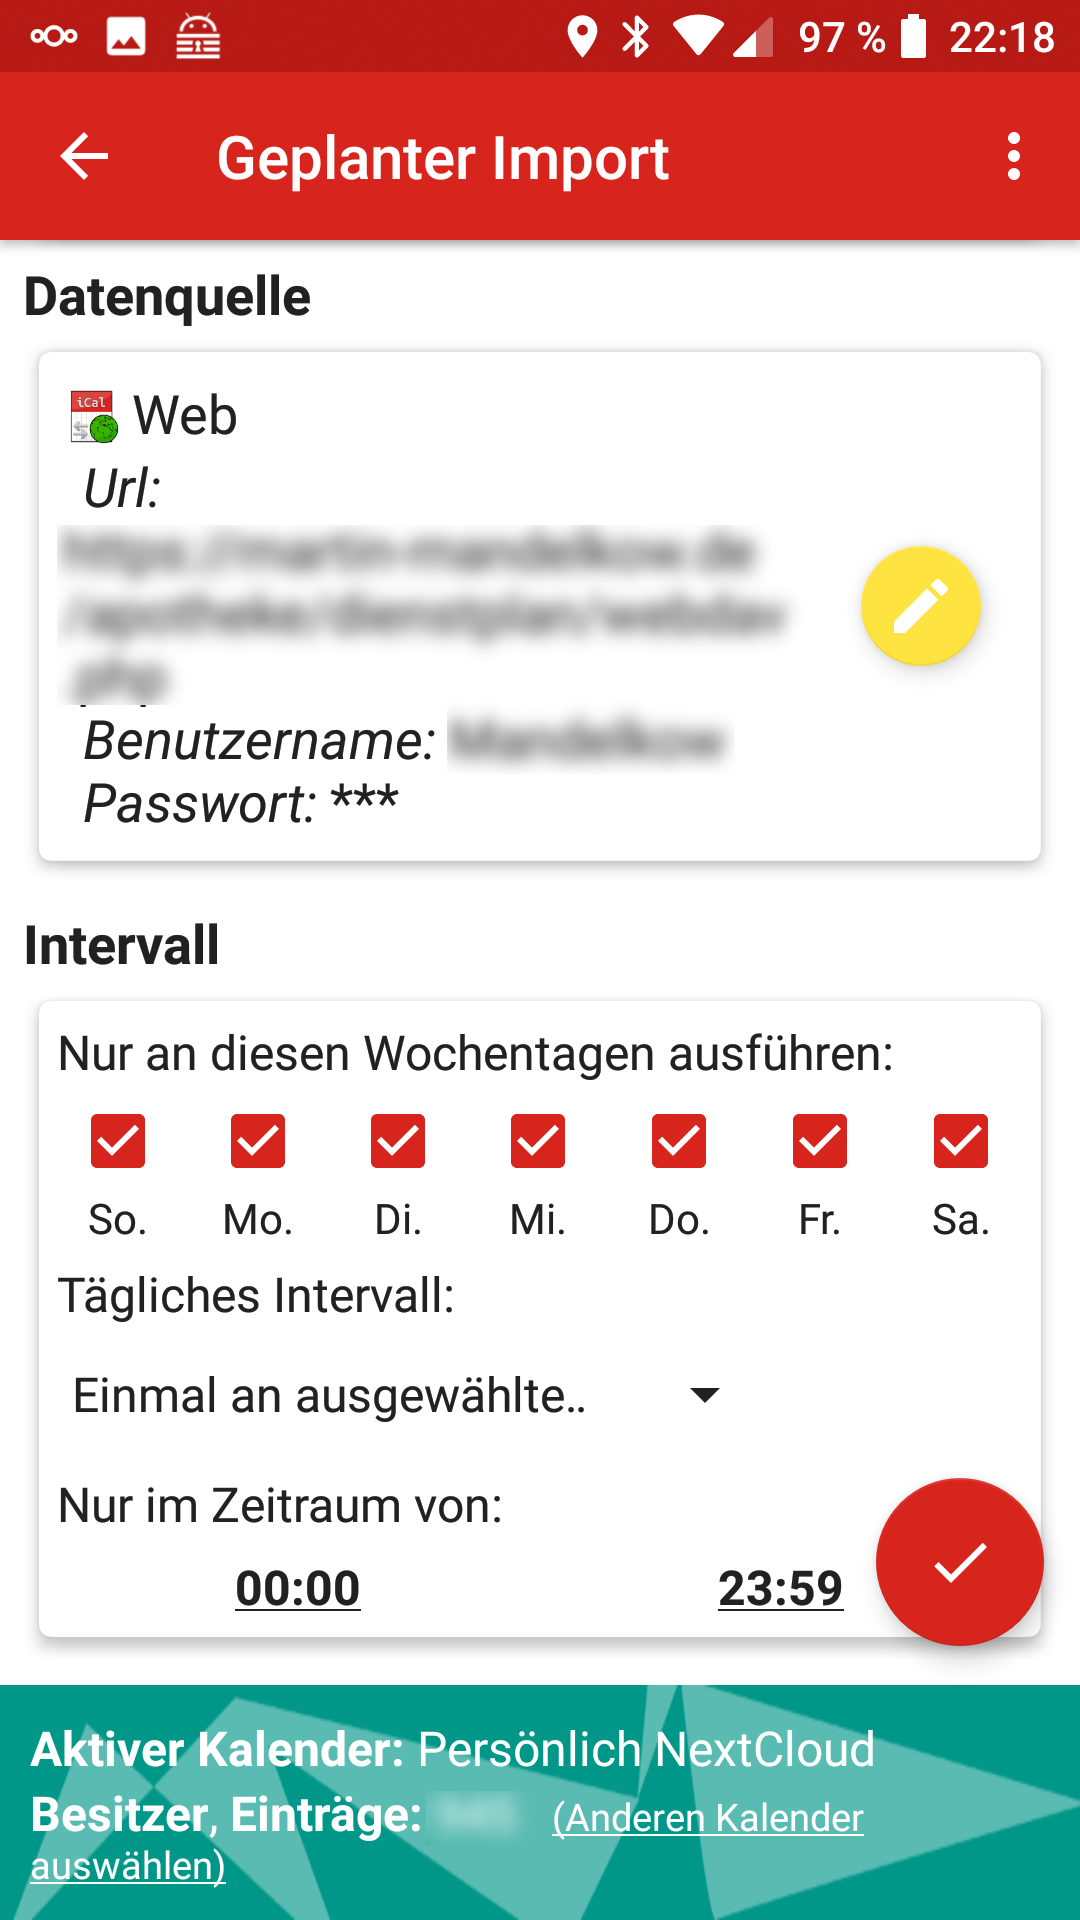
\includegraphics[width=0.9\textwidth, height=0.3\textheight, keepaspectratio=true]{{images/de_DE/iCalendar_import_3.png}}
	\caption{iCal setup import intervals}
    \end{minipage}
    \begin{minipage}{0.45\textwidth}
        \centering
	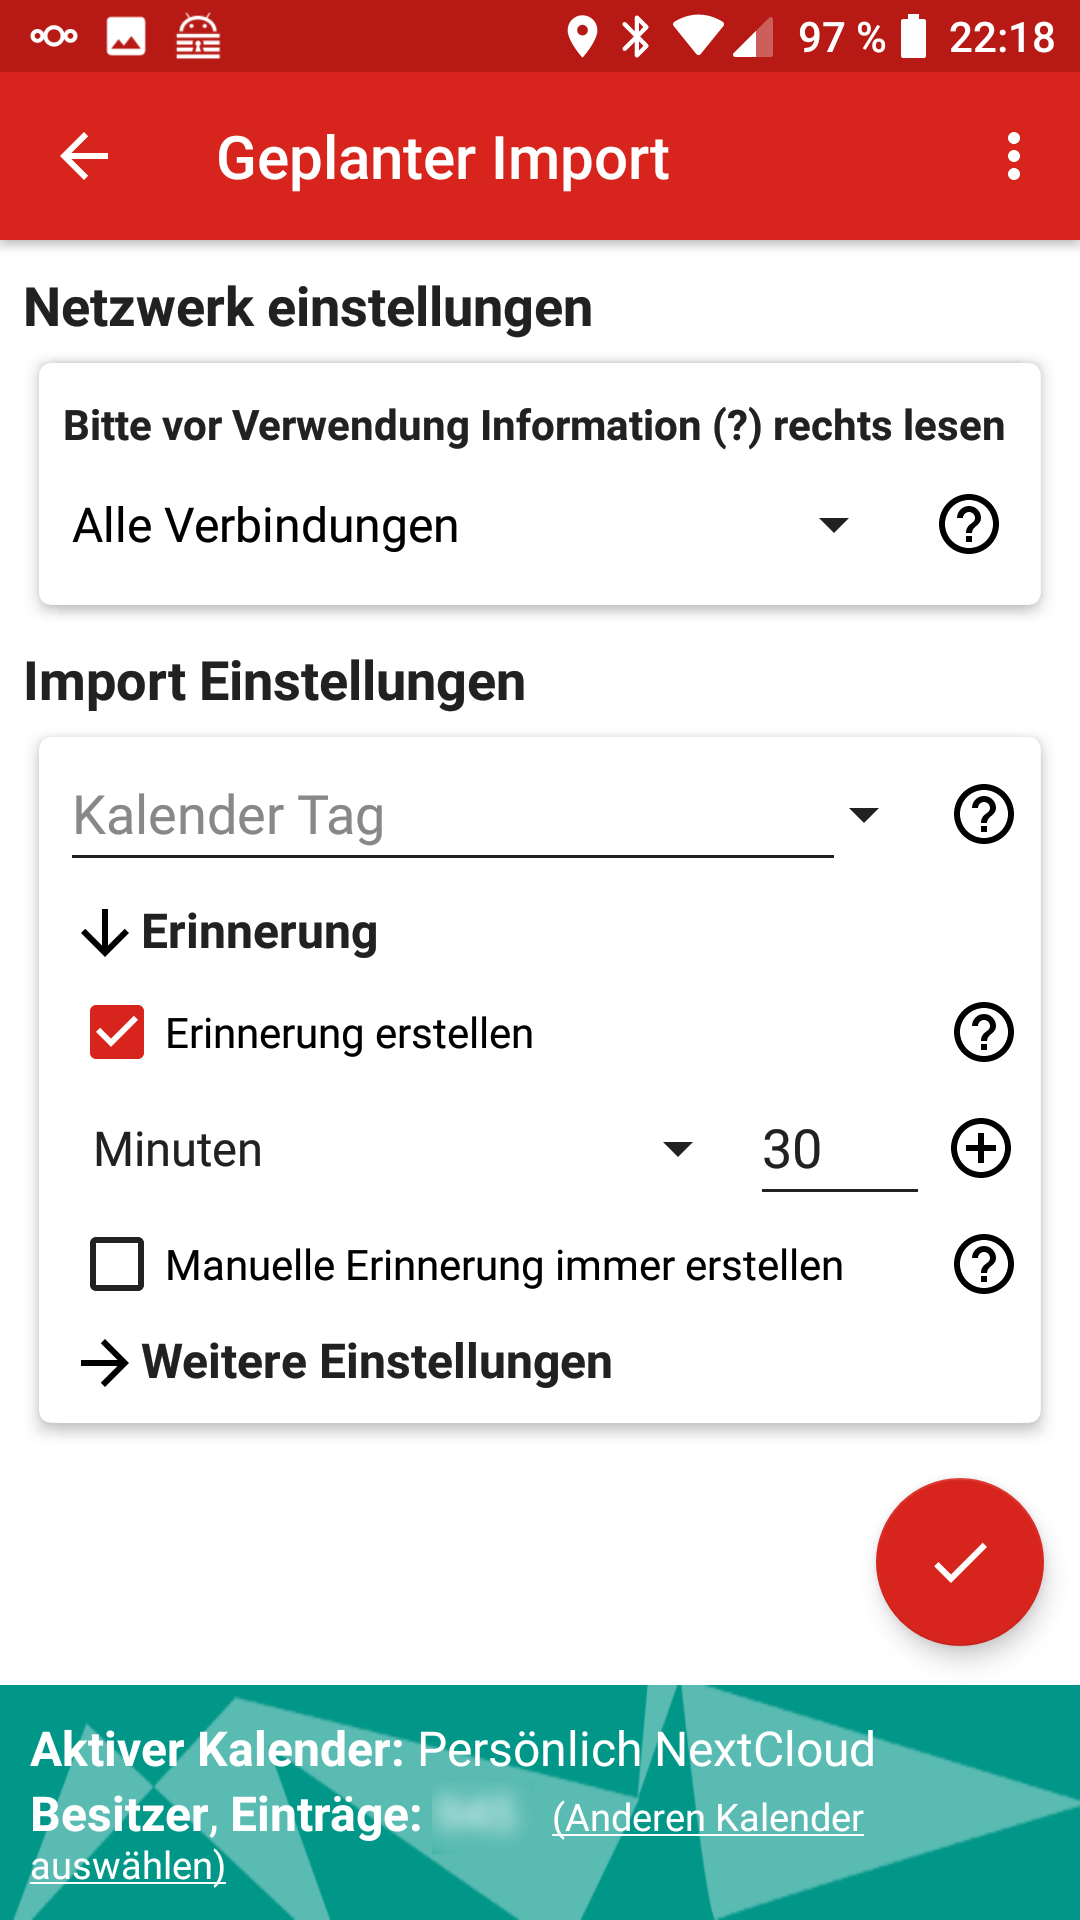
\includegraphics[width=0.9\textwidth, height=0.3\textheight, keepaspectratio=true]{{images/de_DE/iCalendar_import_4.png}}
	\caption{iCal network settings and import settings}
    \end{minipage}
\end{figure}
